
\documentclass{article}
\usepackage{float}
\usepackage{graphicx}
\usepackage{subfig}
\usepackage{lipsum}
\usepackage{tikz}
\usepackage{eso-pic}
\usepackage{changepage}
\usepackage{xcolor}
\usepackage{afterpage}
\usepackage[document]{ragged2e}
\usepackage[none]{hyphenat}
\usepackage[margin=1in,footskip=0.25in]{geometry}
\usepackage{array}
\usepackage{siunitx}
\usepackage{color,soul}
\usepackage{placeins}
\usepackage{siunitx}
\usepackage{microtype}
\usepackage[backend=biber]{biblatex}
\usepackage[hidelinks]{hyperref}
\usepackage[toc,page]{appendix}
\usepackage[toc]{glossaries}
\usepackage[subfigure]{tocloft}
\usepackage{rotating}
\usepackage[printwatermark]{xwatermark}

\cftsetindents{subsection}{.25in}{.4in}

\usepackage[flushleft]{threeparttable}
\newcolumntype{C}[1]{>{\centering\let\newline\\\arraybackslash\hspace{0pt}}m{#1}}

\definecolor{ULred}{HTML}{872434}

\usepackage{chngcntr}
\counterwithin{table}{section}
\counterwithin{figure}{section}

\addbibresource{FireAttackReport.bib}

\setlength{\parskip}{1em}
\pdfoptionpdfminorversion=6

% ******* REMOVE COMMENTS AND PLACE GLOSSARY.TEX IN ROOT DIRECTORY TO ADD GLOSSARY, SEE END FOR ADDITIONAL LINES TO UNCOMMENTS *******
%\loadglsentries{glossary.tex}
%\makeglossaries

% ******* REMOVE COMMENTS ON THIS BLOCK TO ADD DRAFT TO REPORT ********
% \newsavebox\mybox
% \savebox\mybox{\tikz[color=gray,opacity=0.5]\node{DRAFT};}
% \newwatermark*[
% allpages,
% angle=65,
% scale=15,
% xpos=-65,
% ypos=20
% ]{\usebox\mybox}

\begin{document}
	\begin{titlepage}
		
		\pagecolor{ULred}\afterpage{\nopagecolor}
		

		\AddToShipoutPictureFG*{\AtPageUpperLeft{\raisebox{-\height}{
\includegraphics[width=7in]{0_Images/CoverImage.png}}}} 

			\vspace*{23\baselineskip} 

		\huge
		\begin{adjustwidth}{-0.5in}{-0in}
		\color{white}
		\textbf{Enter Report Title \\ Here \\ With End Lines Between Lines\\}
		\end{adjustwidth}
		\begin{adjustwidth}{-0.5in}{}
		\color{white}
		\vspace{.2in}
		\large
		Author 1 \\
		Title 1 \\
		UL Firefighter Safety Research Institue \\
		\vspace*{\baselineskip}
		Author 2\\
		Title 2 \\
		UL Firefighter Safety Research Institute \\ 
		\vspace*{\baselineskip}
		\today
		\vspace*{\baselineskip}
		\vspace{.2in}
		\begin{figure}[h]
			\hspace*{-0.5in}
\includegraphics[width=0.75in]{0_Images/ULLogoWhite.pdf}
		\end{figure}
		\end{adjustwidth}
	\end{titlepage}

\renewcommand{\abstractname}{Executive Summary}
\setlength{\emergencystretch}{5pt}

\begin{abstract}
Text for report Abstract.

\end{abstract}

\newpage

\tableofcontents

\newpage

\section*{Introduction}


\clearpage

\section{Background}

\clearpage

\section{Objectives and Technical Plan}

\subsection {Objectives}



\subsection{Technical Plan}

This study consisted of the following tasks:

\begin{itemize}
	\item Item 1
	\item Item 2
\end{itemize}

\subsection{Limitation and Scope}

\clearpage

\section{Project Technical Panel}

A general discription of the technical panel and the make up.

\begin{figure}[H]
	\centering
	\includegraphics[width = 5in]{} 
	\caption{Positive Pressure Attack Technical Panel Member Locations}
	\label{fig:PanelLocatoins}
\end{figure} 

The individuals below provided direction for the project, assisting in planing the experiments, witnessing the testing and developing tactical considerations. Their tireless support and effort make this project relevant to the fire service across the world. 

\renewcommand{\arraystretch}{1.5}

\begin{table}[H]
	\centering
	\caption{Fire Service Technical Panel}
	\begin{tabular}{|c|c|}
		\hline
		\bf{Name} & \bf{Fire Department} \\ \hline \hline
		Name 1 & Department 1 \\ \hline
		Name 2 & Department 2 \\ \hline
	\end{tabular}
	\label{tab:TechPanelList}
\end{table}

\clearpage

\section{Previous Literature}
\subsection{Fire Service Publications}
\subsection{Fire Service Training Manuals}
\subsection{Firefighter Line of Duty Deaths}
\subsection{Research Work}

\clearpage

\section{Instrumentation}
Throughout this project measurements were taking of temperature, heat flux, pressure, gas velocity and heat release rate. The same instrumentation was utilized for all three sets of experiments. The following describes the instrumentation used and potential uncertainty.

Heat flux measurements were made using a 2.54 cm nominal diameter water-cooled Schmidt- Boelter heat flux gauge (Figure \ref{fig:HeatFluxGauge}). The gauges measured the combined radiative and convective heat flux. For these experiments, the dominant form of heat flux is radiative due to the distance of the heat flux gauges from the flames. It should be noted that the convective contribution to the heat flux is dependent upon the surface temperature of the heat flux gauge. The manufacturer gives an uncertainty of ±3\% and results from a study on heat flux calibration found the typical expanded uncertainty to be ±8\% \cite{HeatFluxRoundRobin}.

\begin{figure} [H]
	\centering
	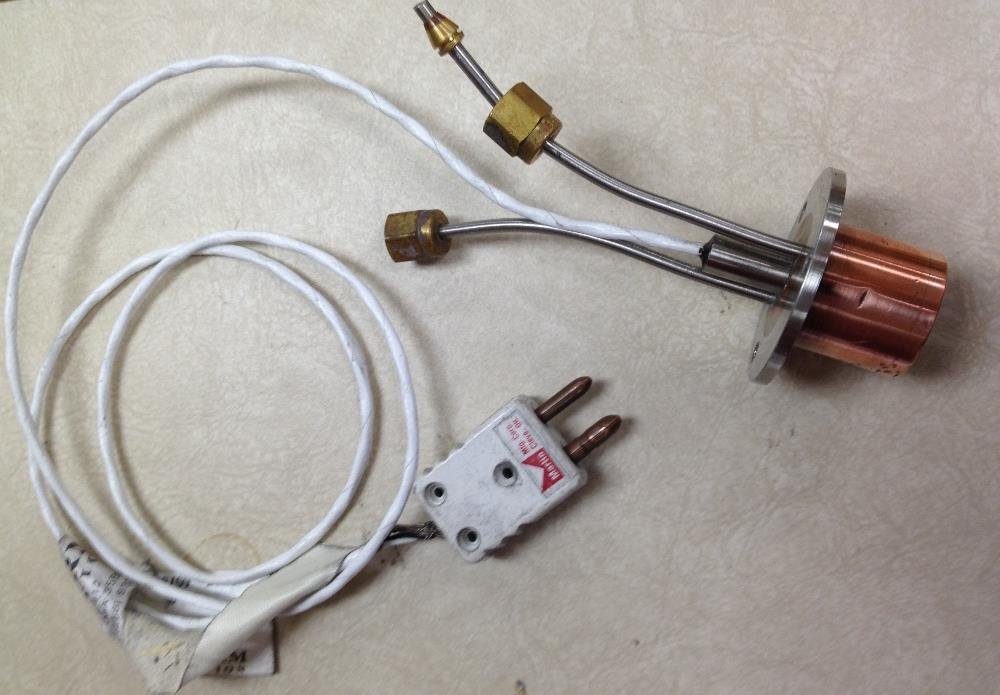
\includegraphics[width = 3.5in]{0_Images/Instrumentation/Heat_Flux_Gauge.jpg}
	\caption{Water Cooled Schmidt-Boelter Heat Flux Gauge}
	\label{fig:HeatFluxGauge}
\end{figure}

Temperatures were recorded using a bare-bead, Chromel-Alumel (type K) thermocouple with a 0.5 mm nominal diameter (Figure \ref{fig:Thermocouple}). The uncertainty given by the manufacturer for the temperature measurements is ±2.2 oC for temperatures below 293 oC and ±0.75\% for higher temperatures \cite{TemperatureHandbook}. The thermocouple readings will be lower than the air temperature when the thermocouple is in the flame region, due to radiative losses to the surrounding cooler environment. When the thermocouples are farther from the flame region, the impact of radiation will result in temperature readings higher than the air temperature. Due to the effect of radiative heat transfer to the thermocouples, the expanded uncertainty is approximately ±15\%.

\begin{figure} [H]
	\centering
	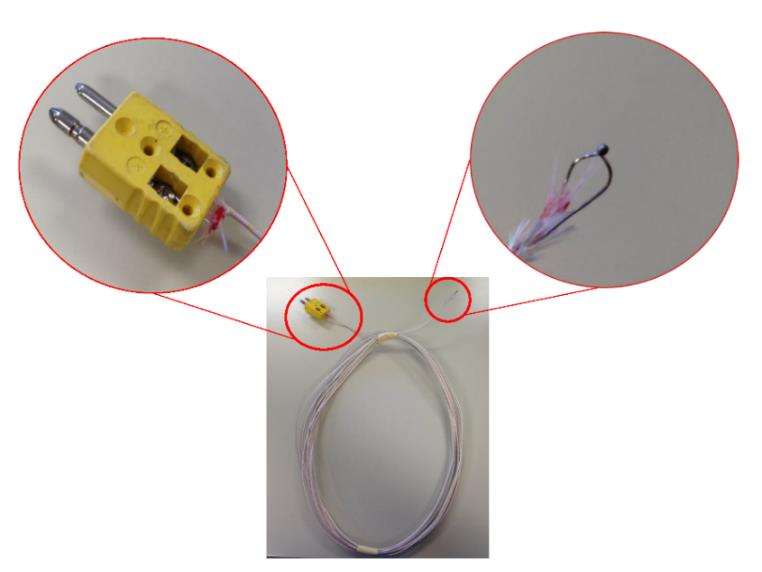
\includegraphics[width = 4in]{0_Images/Instrumentation/Thermocouple.jpg}
	\caption{Chromel-Alumel (Type K) Thermocouple}
	\label{fig:Thermocouple}
\end{figure}

Pressure was recorded through the use of a Setra Model 264 differential pressure transducer with a range of ±0.5” Wc (±124.5 Pa) (Figure \ref{fig:Setra}). The transducer was used to evaluate the pressure difference from ambient pressure. The uncertainty given by the manufacture is ±1\% or ±1.2 Pa \cite{SetraManual}.

\begin{figure} [H]
	\centering
	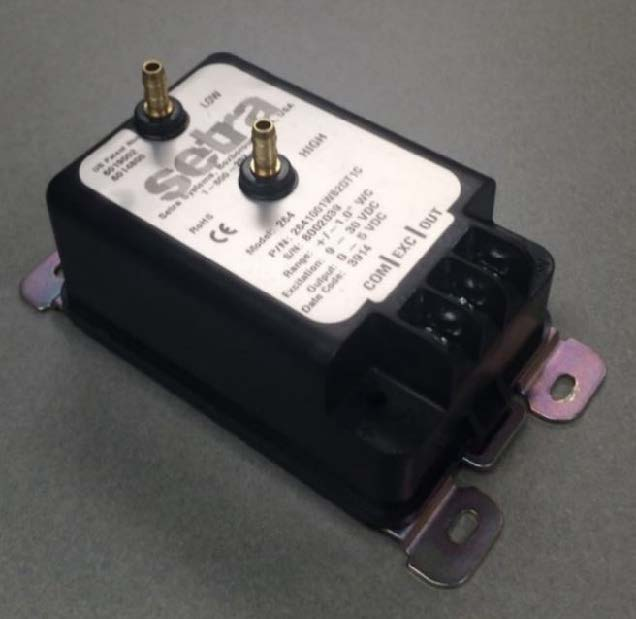
\includegraphics[width = 3in]{0_Images/Instrumentation/Setra.jpg}
	\caption{Setra Model 264 Differential Pressure Transducer}
	\label{fig:Setra}
\end{figure}

Gas velocity was obtained through the use of a bi-directional probe in conjunction with a differential pressure transducer and iconel thermocouple. The probe was constructed of stainless steel. The iconel thermocouple was a 0.063in. diameter type KSL iconel 600 sheathed grounded junction with a type K, 24 gauge glass/glass insulation lead. The differential pressure transducer was a Setra Model 264 with a \hl{range of ±1.0in. WC (±248.8 Pa) CORRECT FOR ACTUAL RANGE}. The configuration had a velocity range of \hl{±24.2 m/s (±54 mph) CORRECT FOR ACTUAL RANGE}. The pressure transducers were configured in groups of 6, contained in a single plastic box with connections for pressure, temperature and power (Figure \ref{fig:BDP})b. Five probes were installed in openings where velocity measurements were taken, centered horizontally in the opening (Figure \ref{fig:BDP}a). Velocity measurement with this configuration was determined to have an uncertainty of ±5\% \cite{BDPInPoolFires}.

\begin{figure} [H]
	\centering
	\begin{tabular}{c c}
		\subfloat[Pressure Transducer Box]{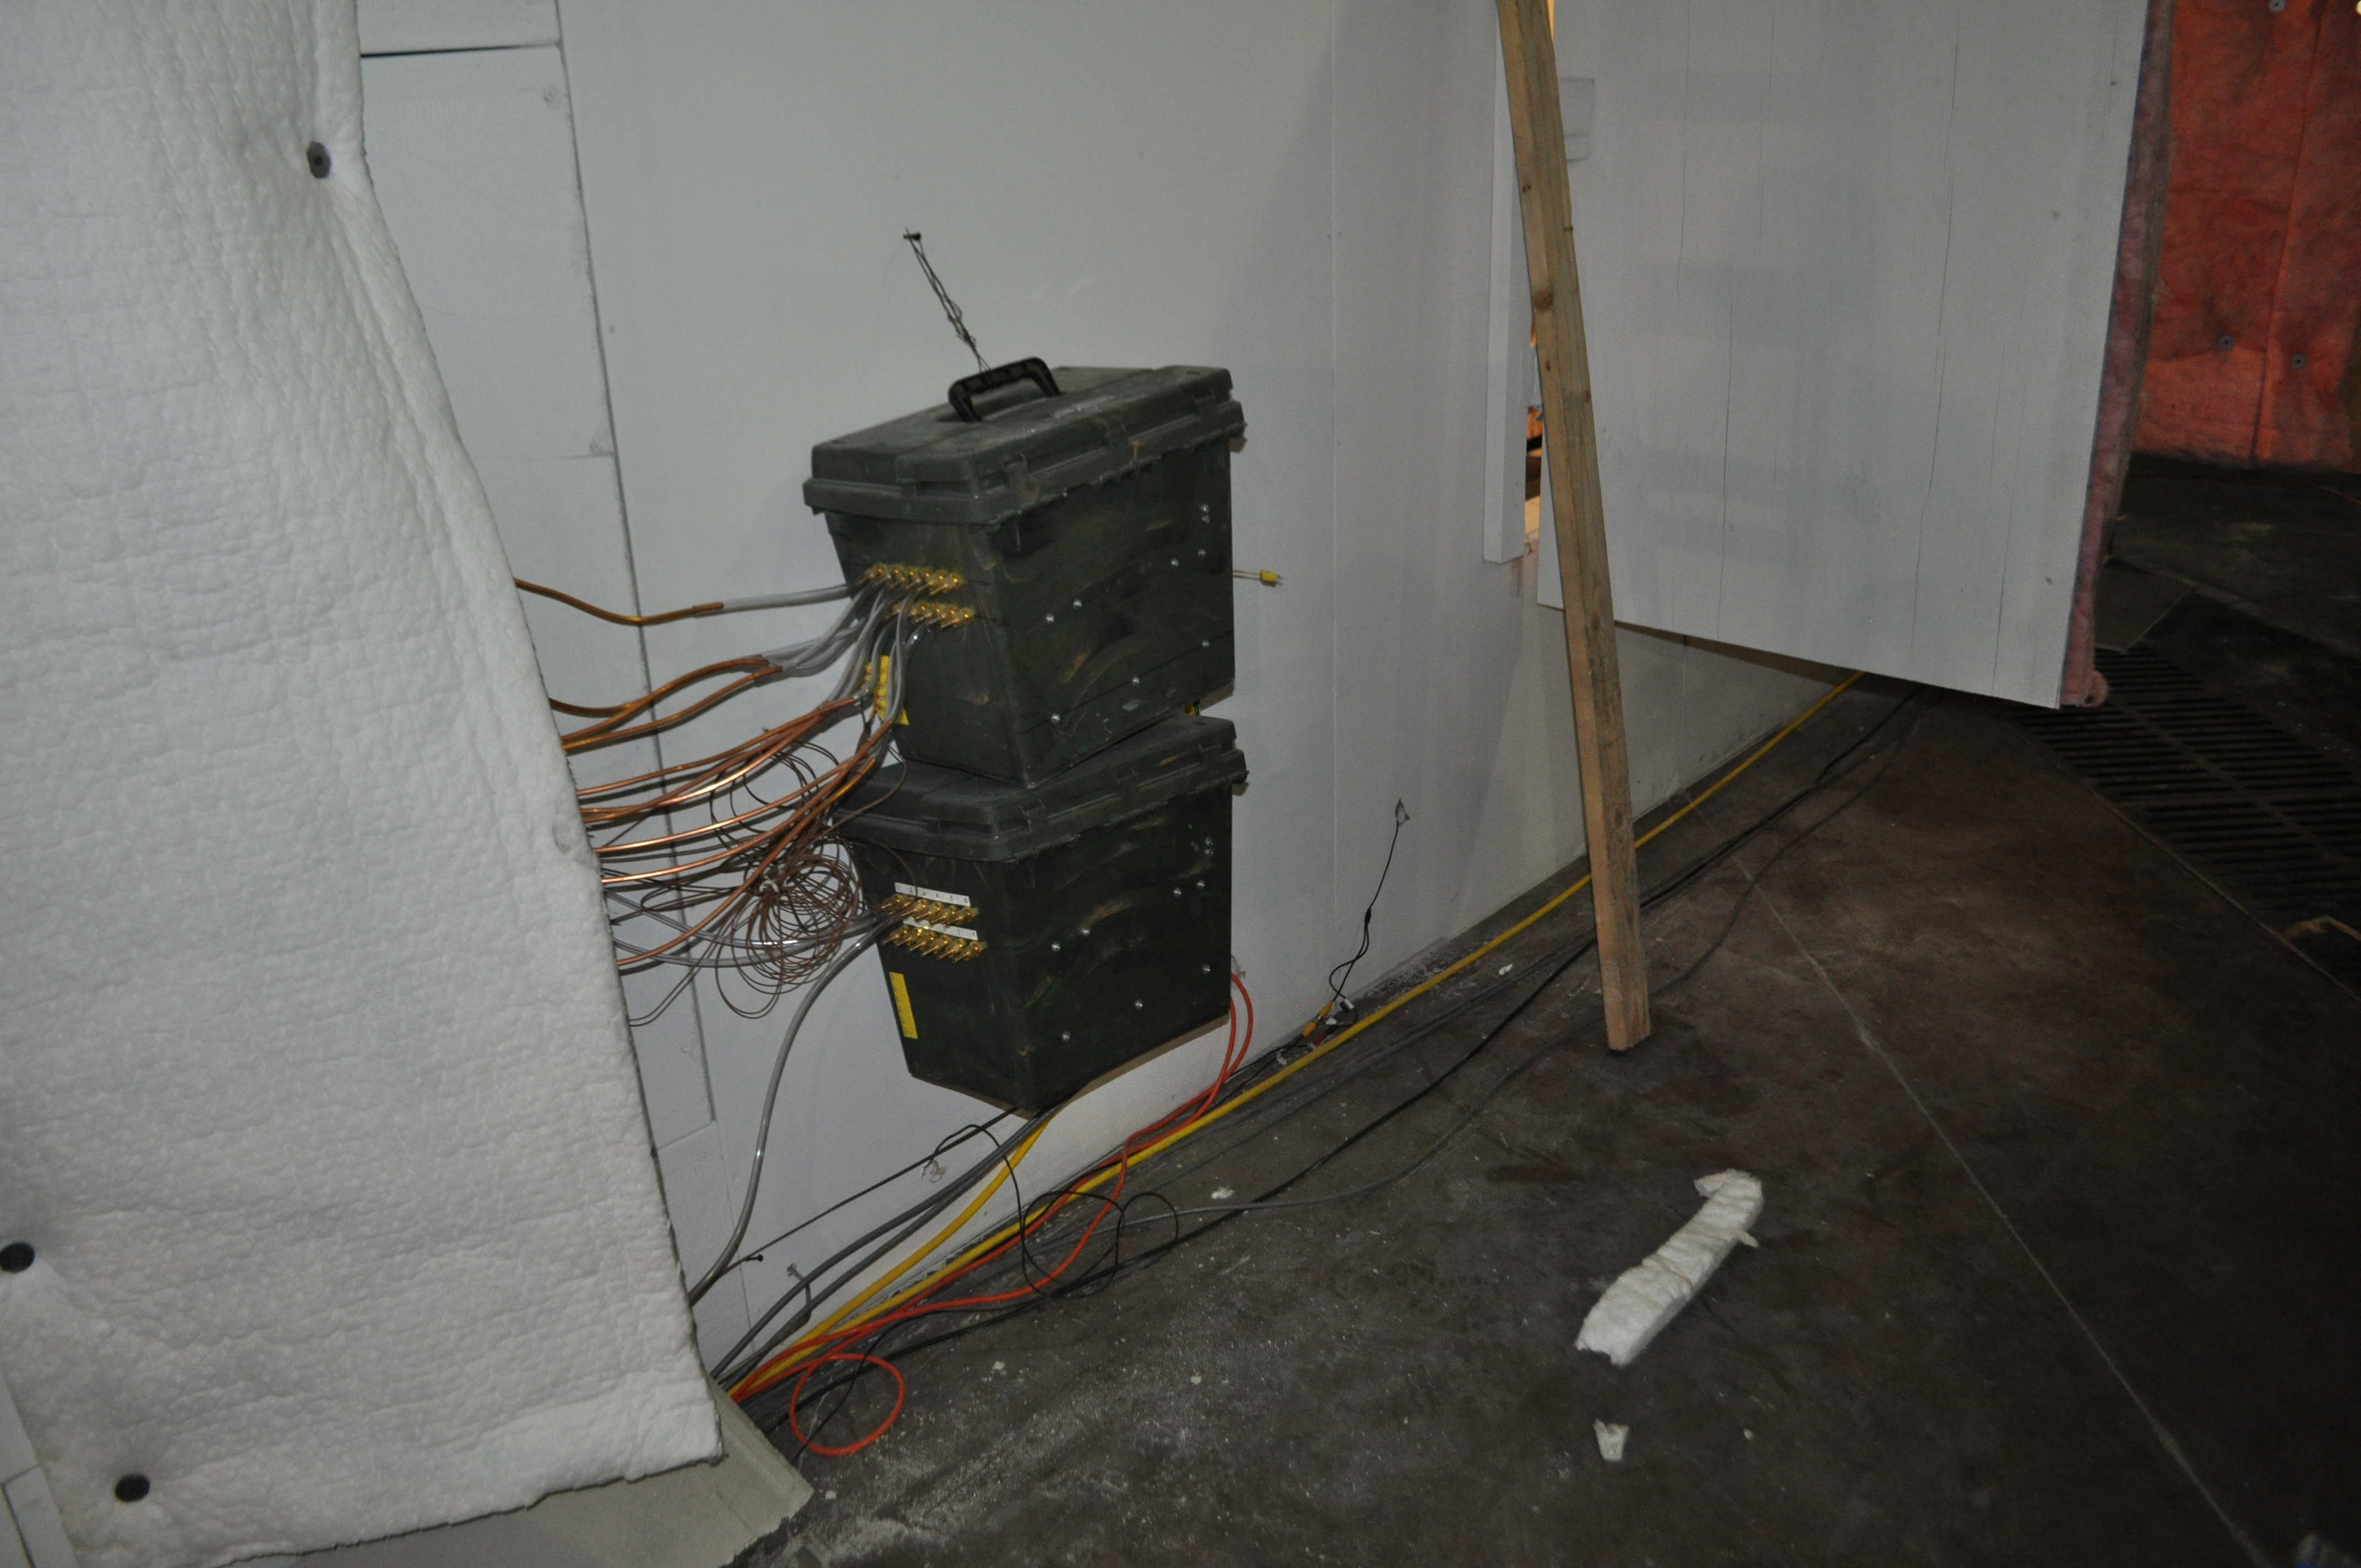
\includegraphics[height = 2.5in]{0_Images/Instrumentation/PressureBox.jpg}} &
		\subfloat[Bi-Directional Probe Array]{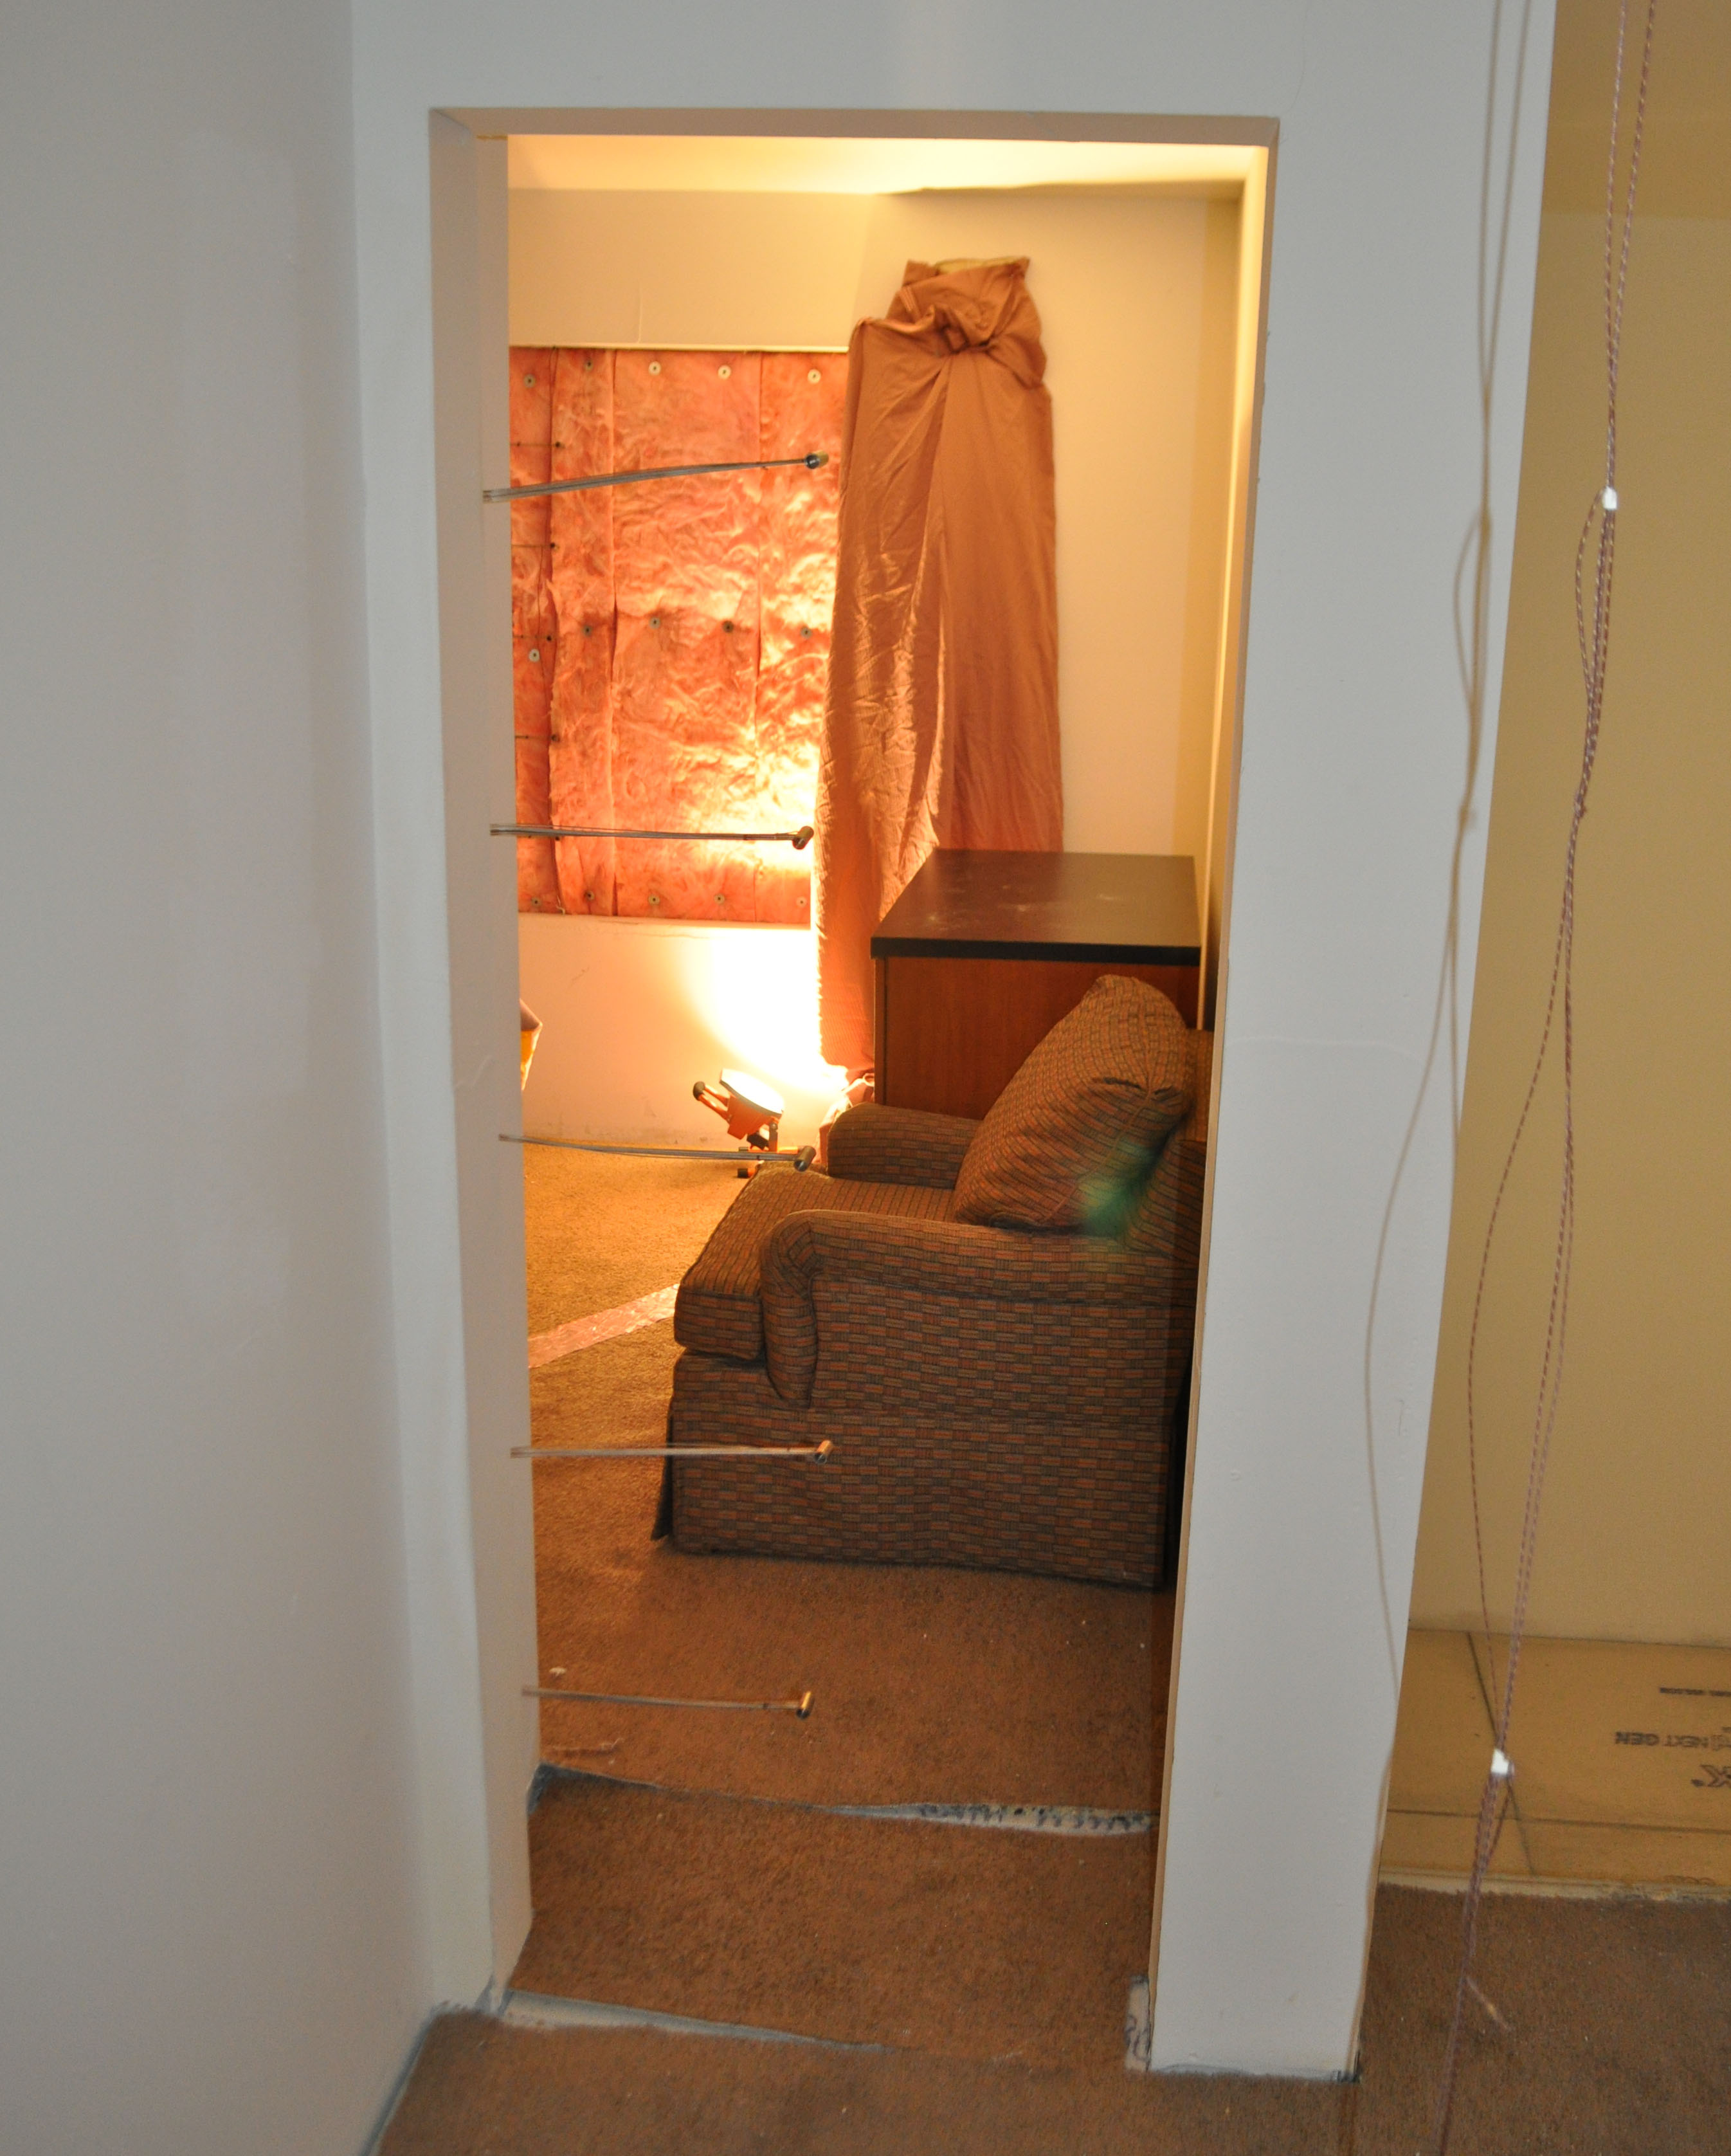
\includegraphics[height = 2.5in]{0_Images/Instrumentation/BDPArray.jpg}} \\
	\end{tabular}
	\caption{Bi-Directional Probe}
	\label{fig:BDP}
\end{figure}

The heat release rate is measured through the use of oxygen consumption techniques. The oxygen consumption calorimeter is capable of accurately measuring the heat release rate up to 10 MW. Above 10 MW, larger inaccuracies are expected due to the combustion products overflowing the collection hood. Figure \ref{fig:Hood} shows the collection hood utilized for the calorimetry data.

\begin{figure} [H]
	\centering
	\includegraphics[width = 5in]{0_Images/Instrumentation/Calorimetry_hood.jpg}
	\caption{Oxygen Consumption Calorimetry Hood}
	\label{fig:Hood}
\end{figure}

Stand video was obtained through the use of BoschVTC-206F03-4 video cameras (Figure \ref{fig:BullettCam}). Thermal imaging of the front and rear of the structure was taken using ISG Infrasys Elite XR (Figure \ref{fig:IRCam}). The thermal imaging camera has a fixed emissivity value of 0.9 and was utilized for visual representation of relative conditions, no temperature measurements or analysis were derived using the camera. All cameras were recorded using a TriCaster 8200 video acquisition system.

\begin{figure} [H]
	\centering
	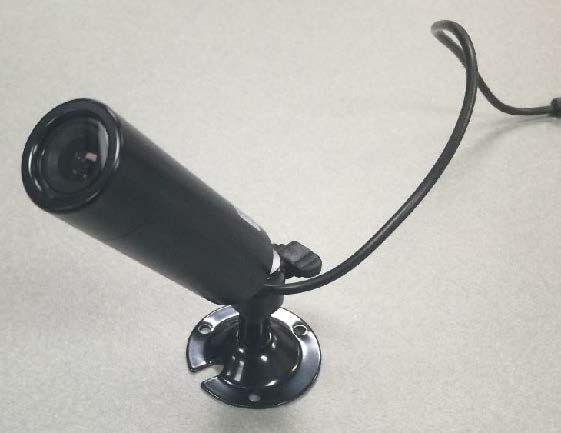
\includegraphics[width = 3in]{0_Images/Instrumentation/BullettCam.jpg}
	\caption{Oxygen Consumption Calorimetry Hood}
	\label{fig:BullettCam}
\end{figure}

\begin{figure} [H]
	\centering
	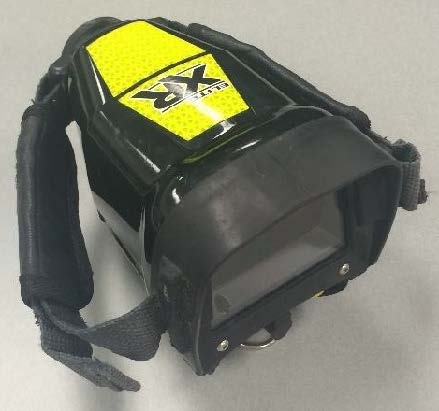
\includegraphics[width = 2.5in]{0_Images/Instrumentation/ISG_IR.jpg}
	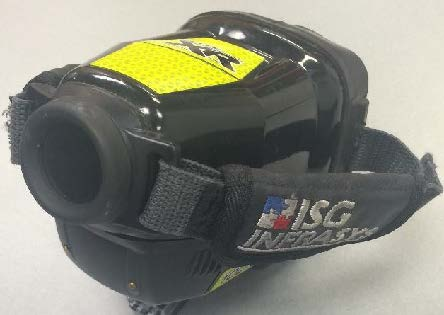
\includegraphics[width = 2.5in]{0_Images/Instrumentation/ISG_IR2.jpg}
	\caption{ISG Elite XR Fire Service Thermal Imaging Camera}
	\label{fig:IRCam}
\end{figure}

Gas samples were analyzed through the use of OxyMat6 and UltraMat23 Siemens gas analyzers. Samples were pulled from the structure through the use of cole palmer model L-79200-30 vacuum/pressure diaphragm pump rated at 0.75CFM via a stainless steel tube. The sample is filtered through a course filter, solberg model 842, 2 micron paper filter before running through a condensing trap to remove moisture. The sample then runs through a drying tube dry fine filter, perma pure model FF-250-SG-2.5G with a 1micron filter FF-250-E-2.5G before splitting into two branches and entering the UltraMat and OxyMat analyzer. The analyzers are calibrated to measure CO from 0-50000PPM, CO2 from 0-20\% and O$_2$ from 0-25\%. 

\begin{figure}[H]
	\centering
	\begin{tabular}{*3c}
		\subfloat[Sample Line]{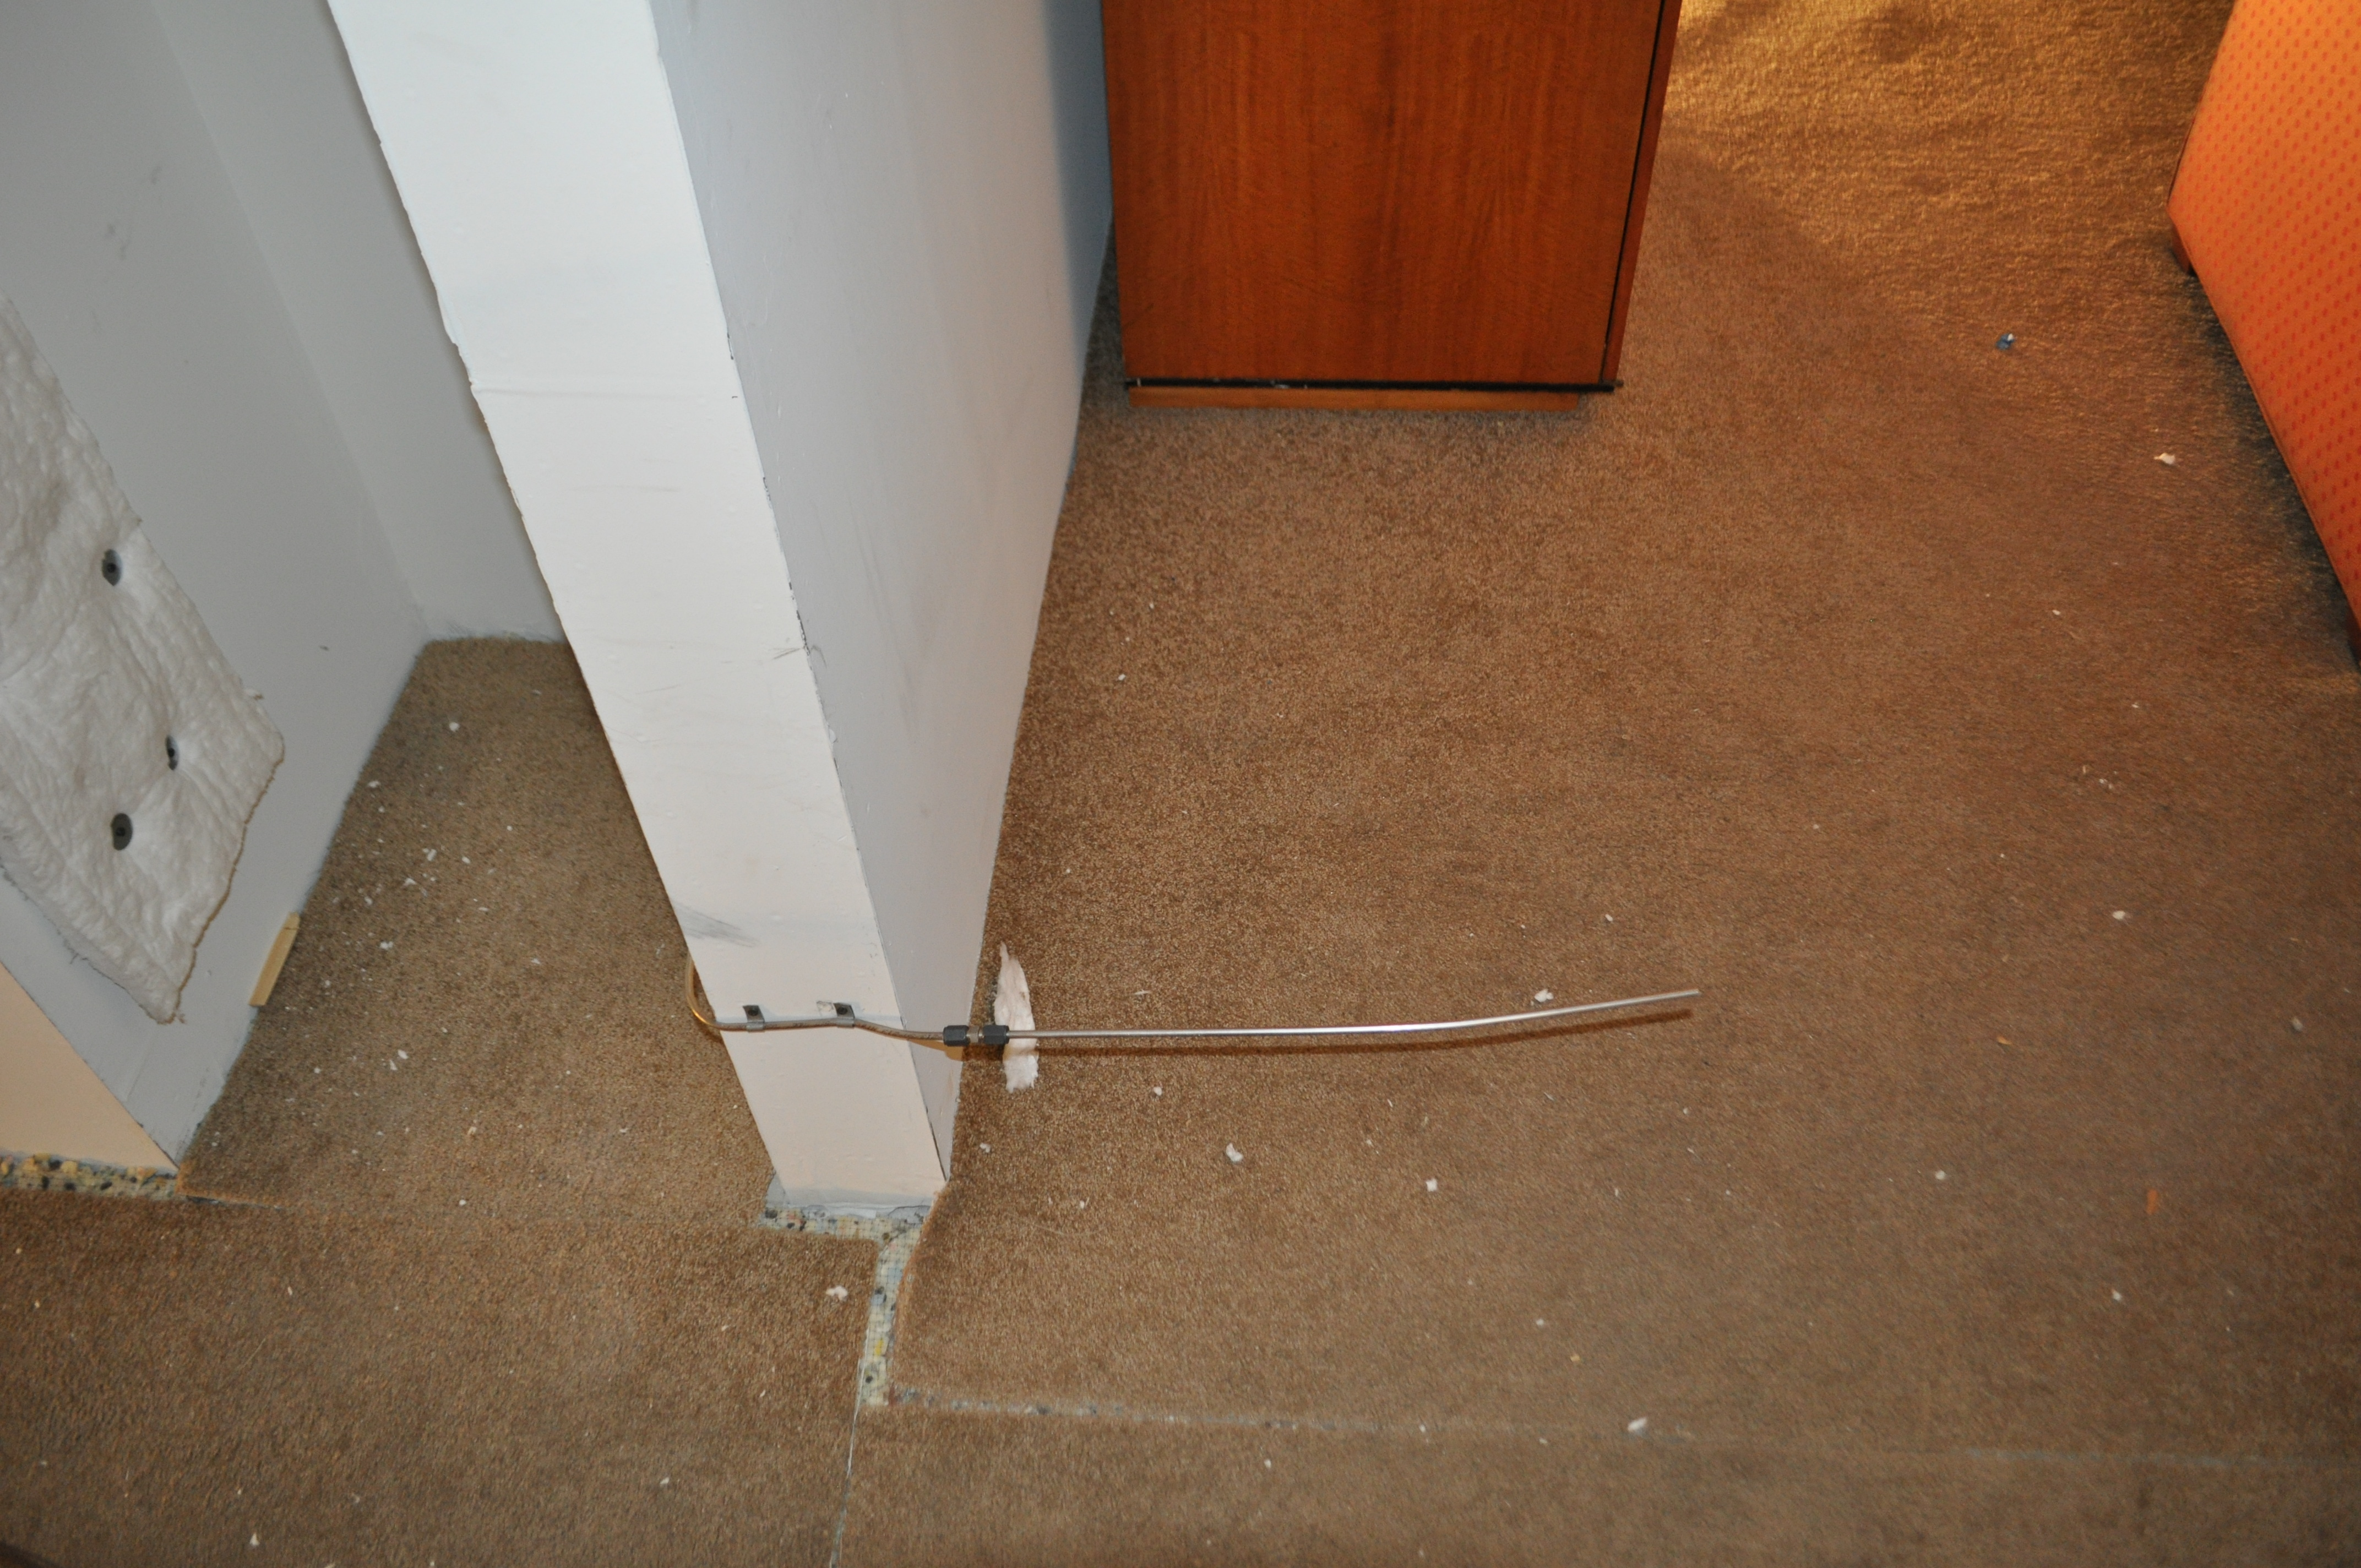
\includegraphics[width = 2in]{0_Images/Instrumentation/Gas_Analyzer/SamplePoint.jpg}} &
		\subfloat[Vaccum Pump - Cole Palmber L-79200-30]{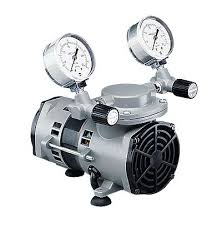
\includegraphics[width = 2in]{0_Images/Instrumentation/Gas_Analyzer/VaccumPump.jpg}} &
		\subfloat[Course Filter - Solberg 842]{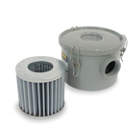
\includegraphics[width = 2in]{0_Images/Instrumentation/Gas_Analyzer/CourseFilter.jpg}} \\
		\subfloat[Condensing Tube]{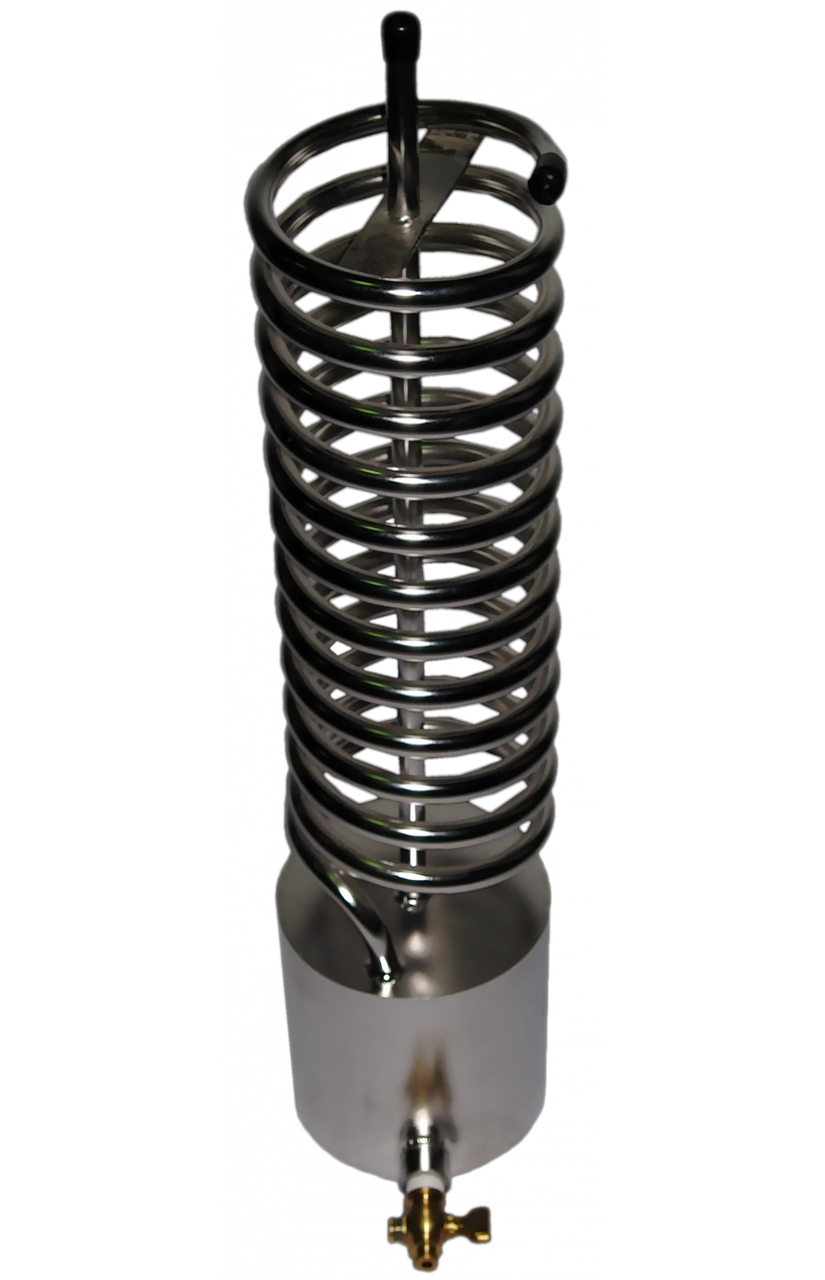
\includegraphics[height = 2in]{0_Images/Instrumentation/Gas_Analyzer/CoilCondenser.png}} &
		\subfloat[Dririte Tube]{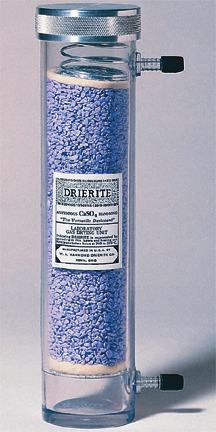
\includegraphics[height = 2in]{0_Images/Instrumentation/Gas_Analyzer/DriRightTube.jpg}} &
		\subfloat[Fine Filter - Perma Pure FF-250-SG-2.5G]{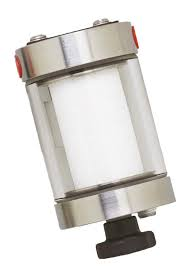
\includegraphics[height = 2in]{0_Images/Instrumentation/Gas_Analyzer/FineFilter.jpg}} \\
	\end{tabular}
	\subfloat[Gas Analyzers]{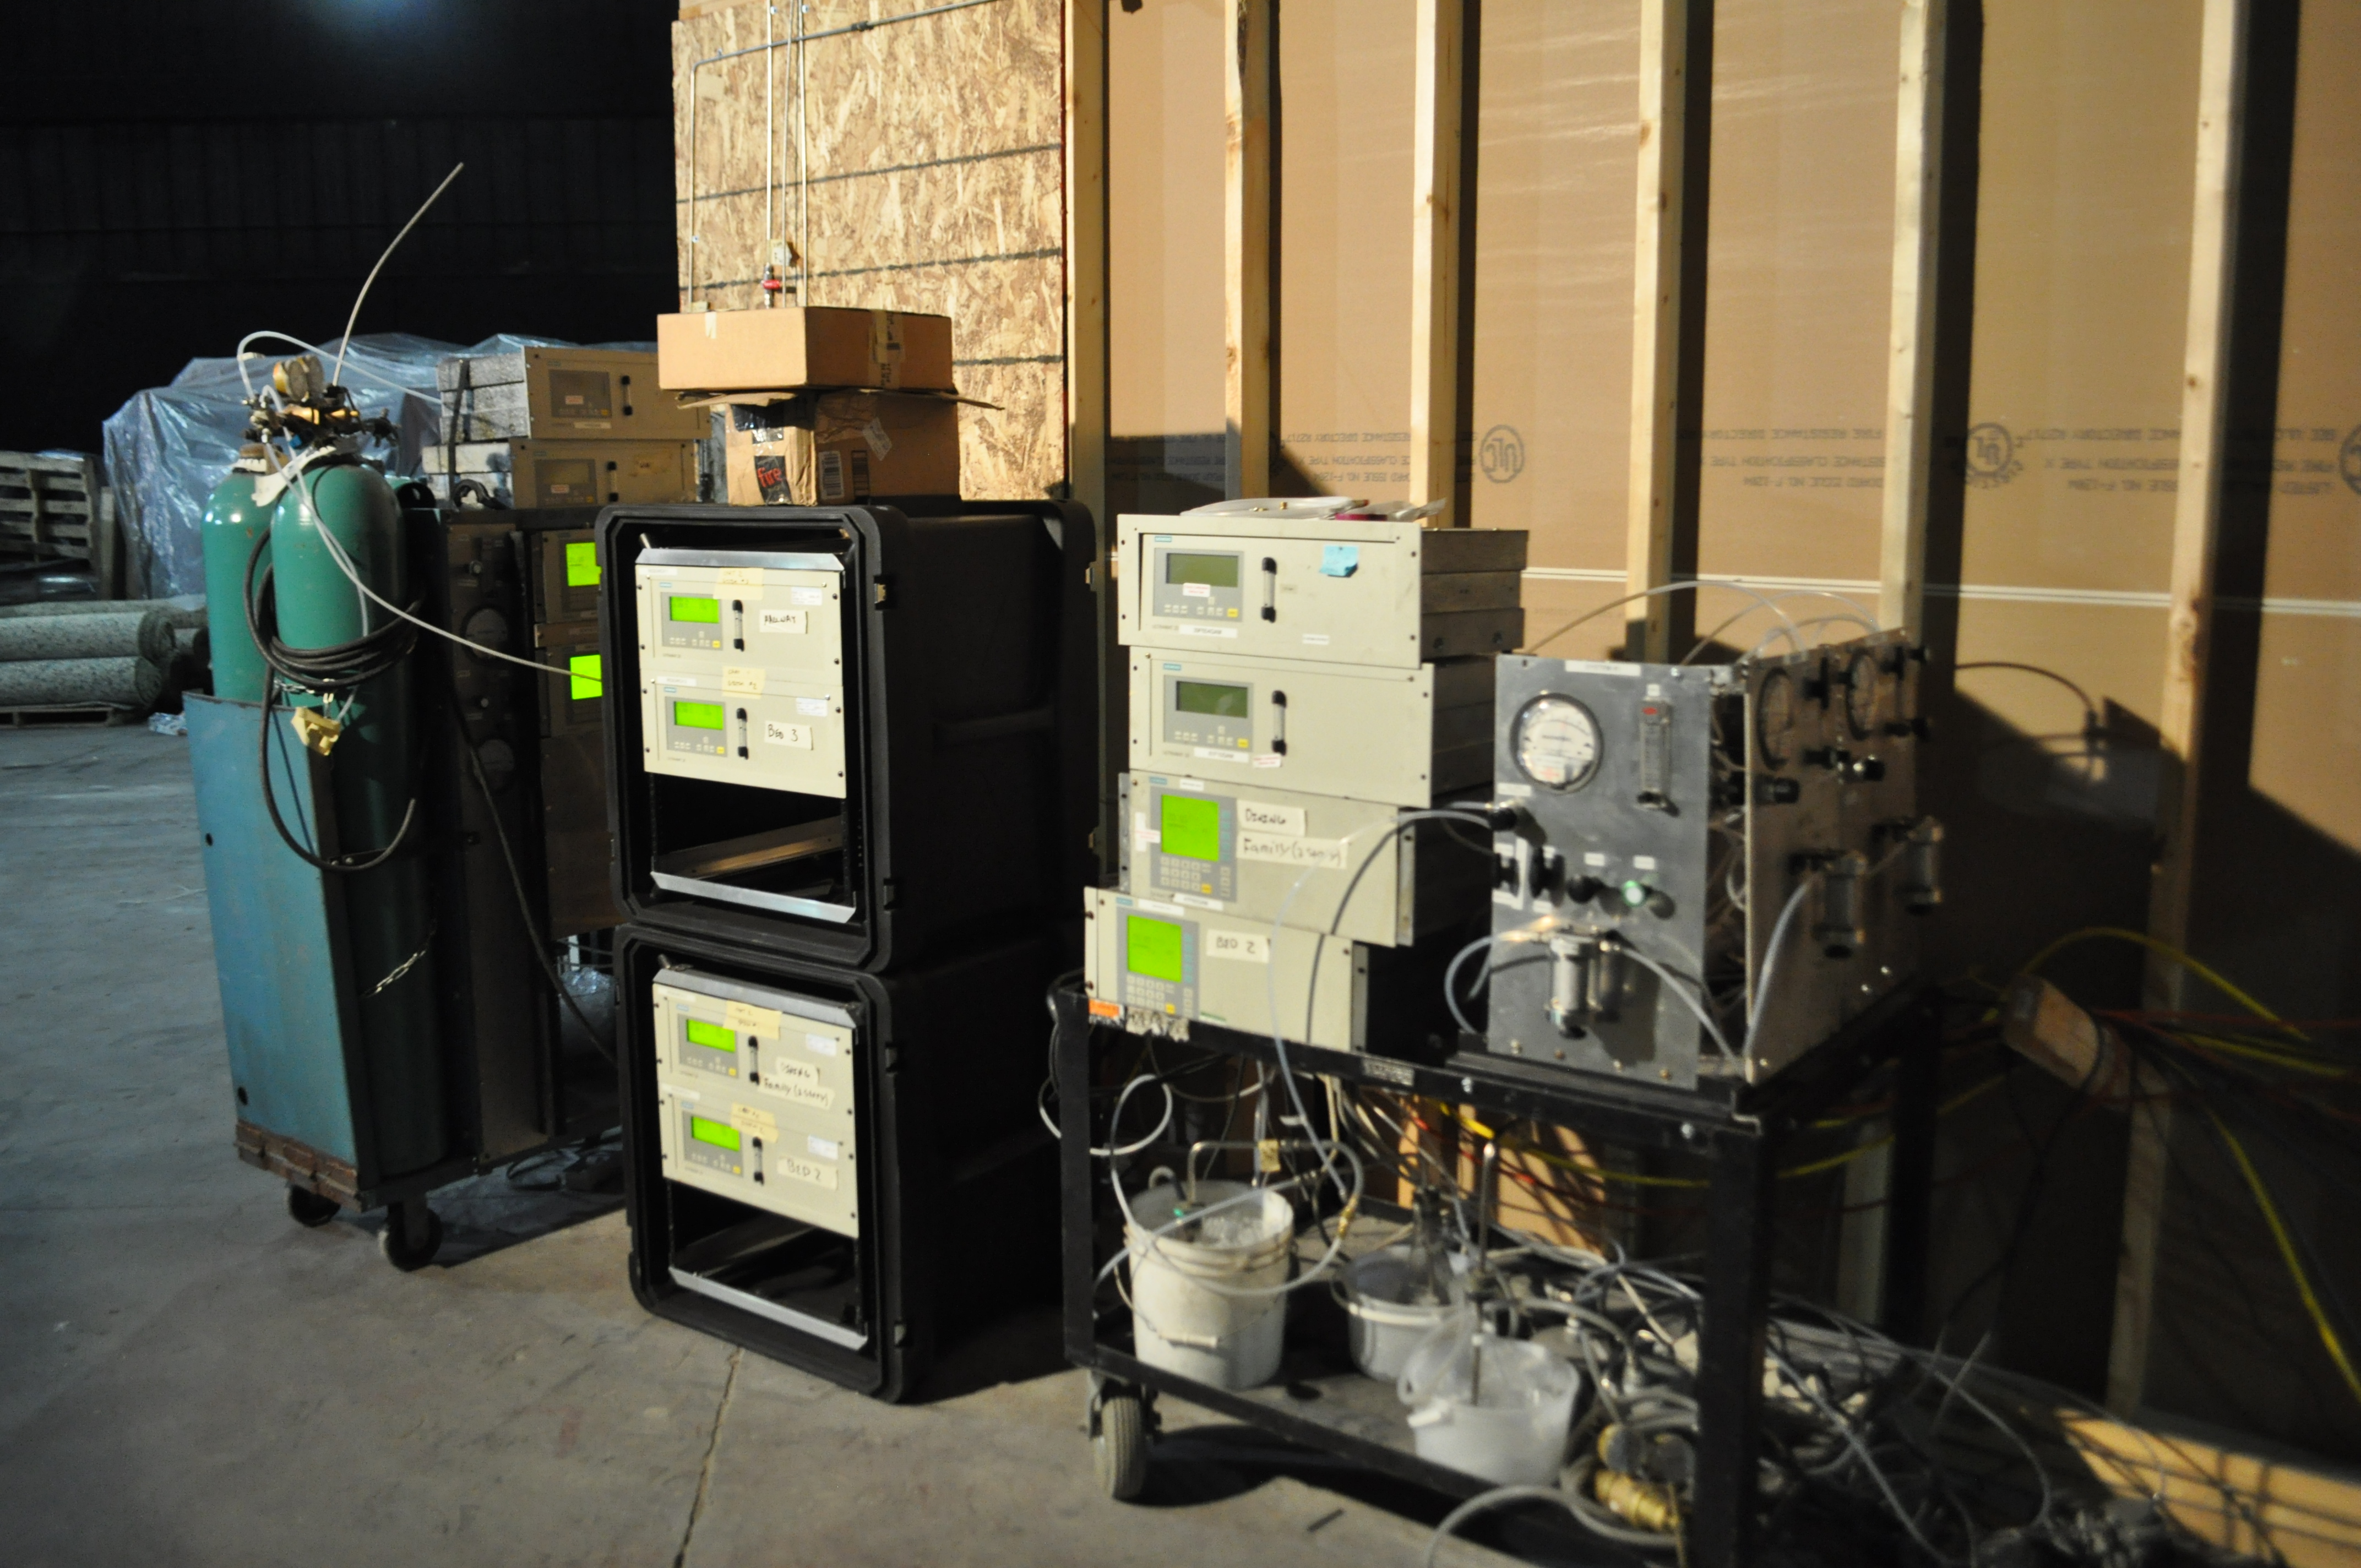
\includegraphics[width = 2in]{0_Images/Instrumentation/Gas_Analyzer/GasAnalyzers.jpg}}
	\caption{Gas Analyzer Configuration}
	\label{fig:GasAnalyzers}
\end{figure}

All data was logged through the use of a national instruments data acquisition system incorporating a SCXI-1001 chassis with 8 SCXI-1102C 32-Channel modules (Figure \ref{fig:DataSystem}). The system is configured for a total of 256 channels capable of reading values between 0-10 volts DC. Values are recorded once a second and translated to quantities of interest through the use of LabVIEW software specifically programmed for use with the system.

\begin{figure}[H]
	\centering
	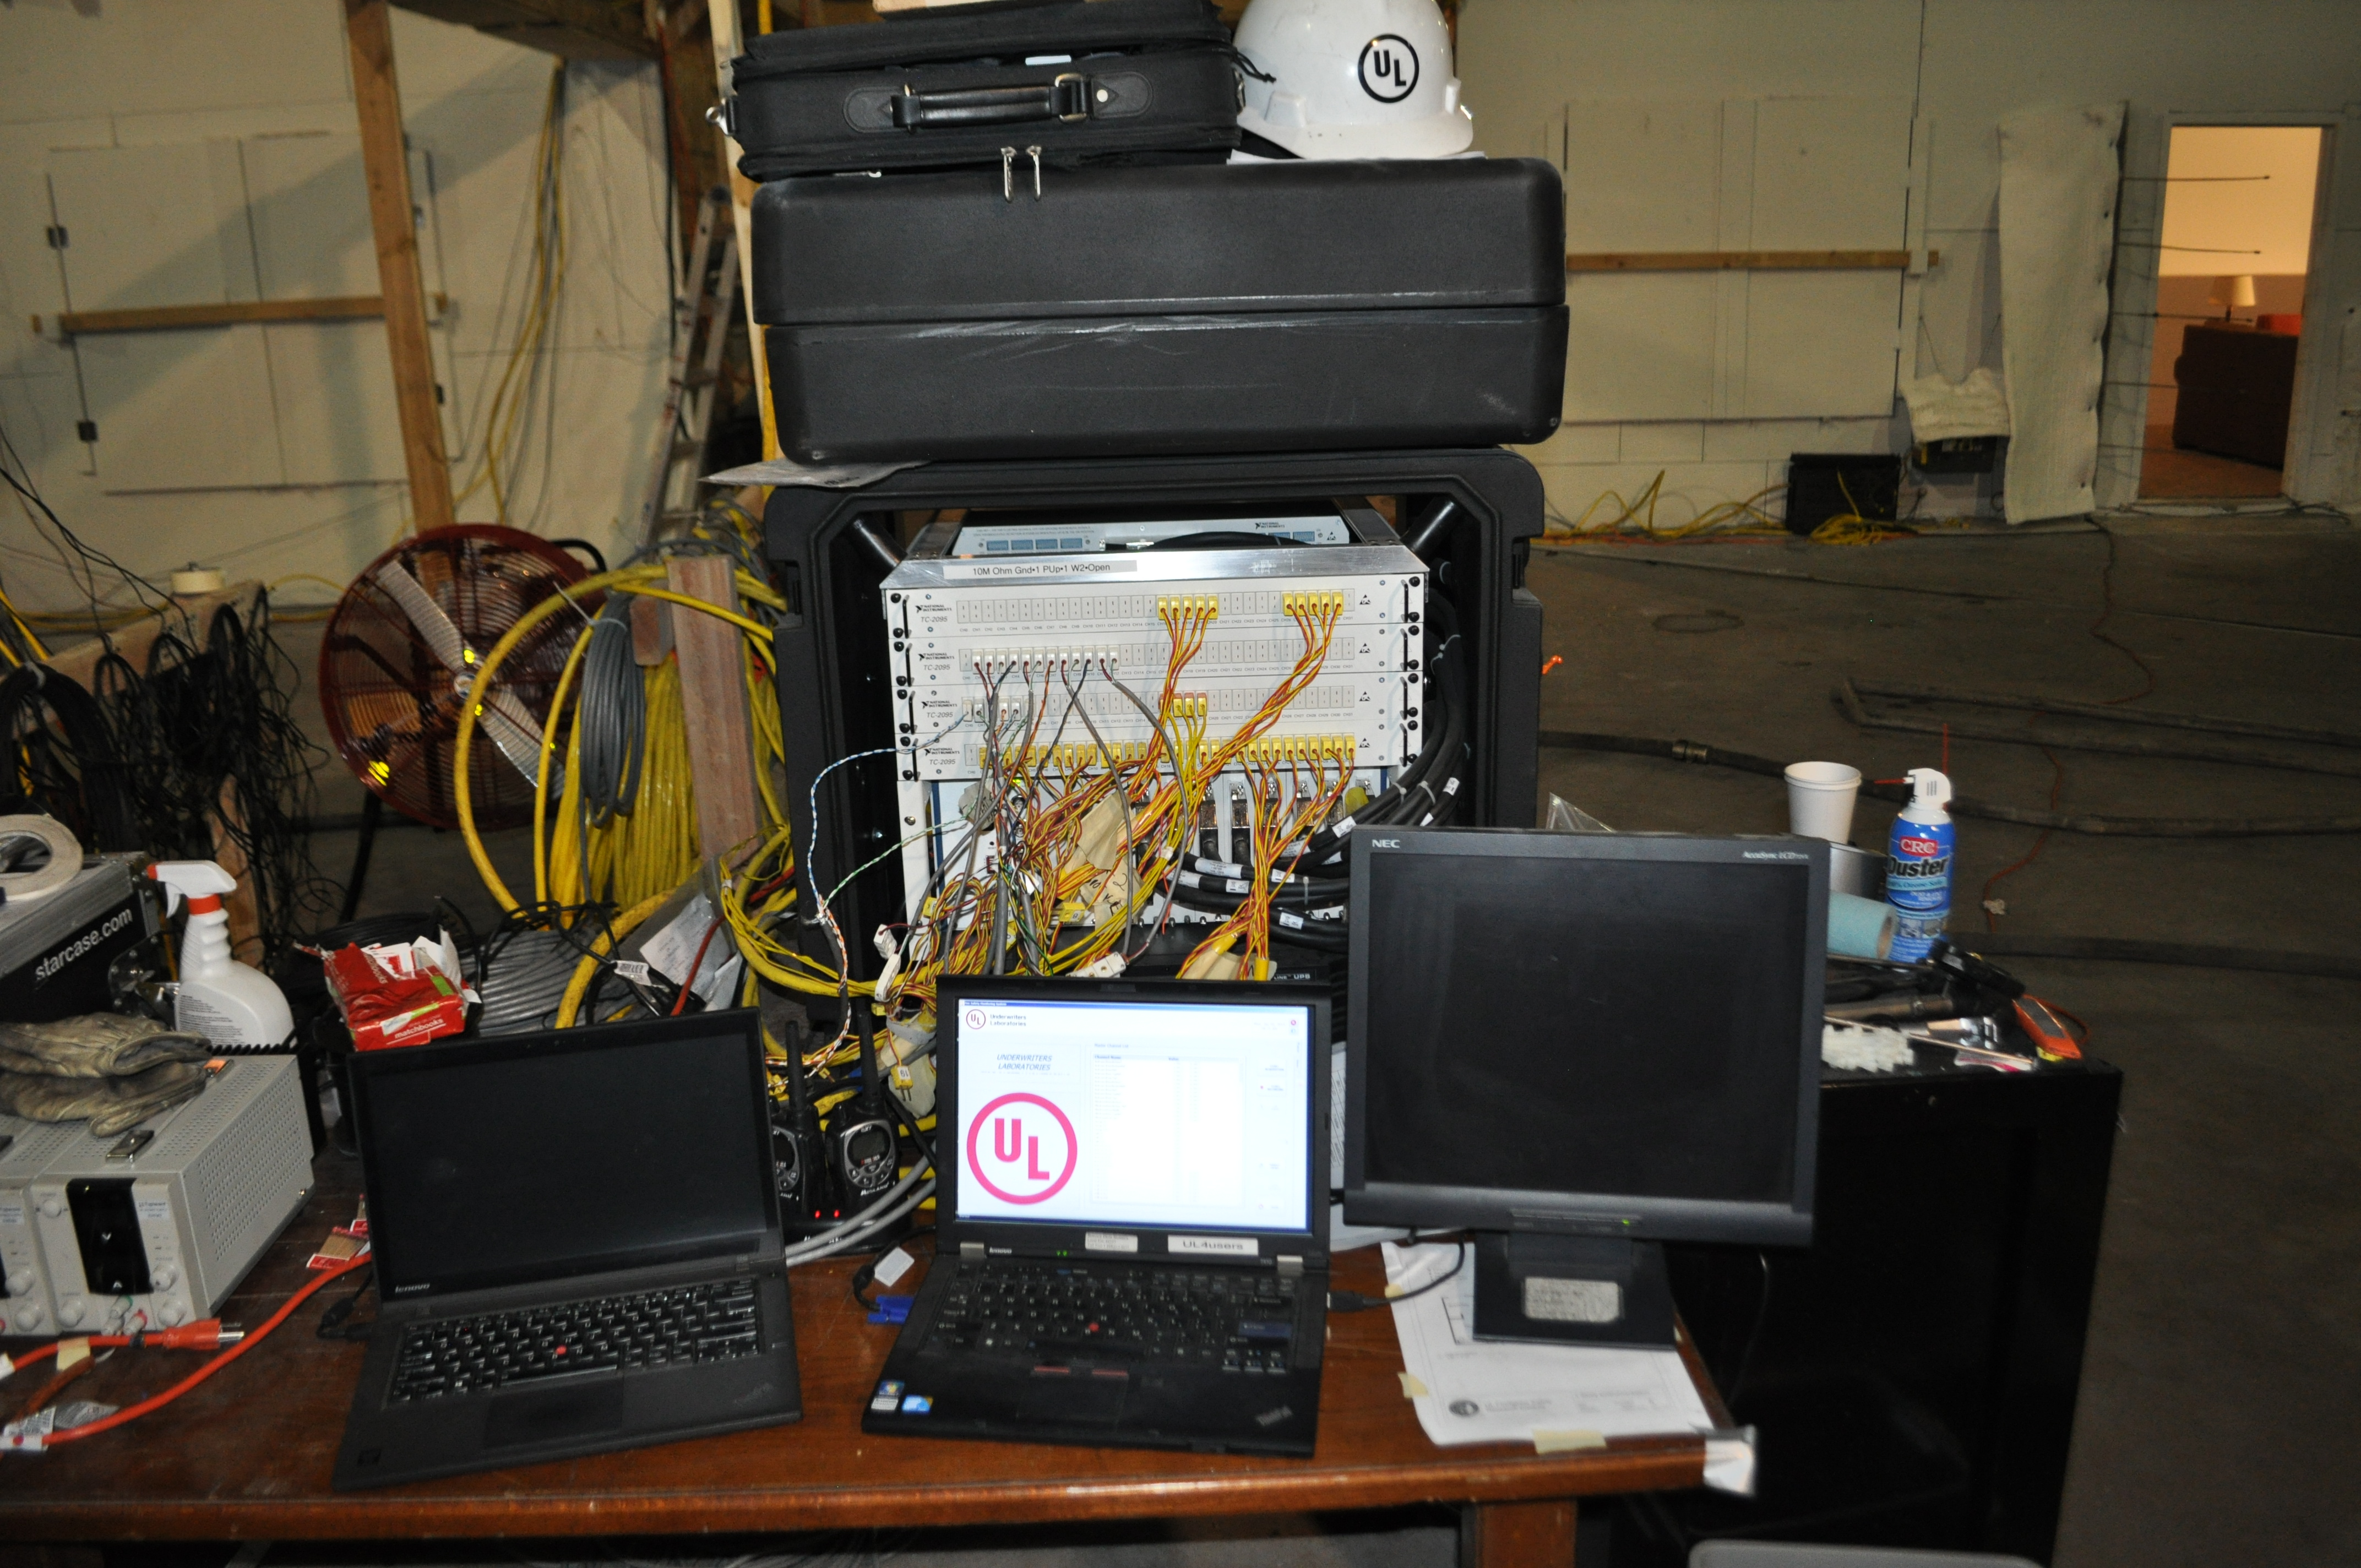
\includegraphics[width = 4in]{0_Images/Instrumentation/DataSystem.jpg}
	\caption{Data Acquisition System}
	\label{fig:DataSystem}
\end{figure}

\clearpage

\section{Test Set Up}

\subsection{Structures}

\subsection{Measurement Locations}

\section{\hl{REMOVE IF NOT APPLICABLE} - Heat Release Fuel Load Characterization} \mbox{}

To characterize the foam furniture energy release rates, heat release rate burns were conducted under a cone calorimeter hood. 

\section{Task 1 Experiments}
\hl{A discription of the experiments.} Table \ref{table:Task_1_Experiments} shows the experiments conducted. 

\begin{table}[H]
	\centering
	\caption{Table Caption}
	\begin{tabular}{|c|c|c|}
		\hline
		Item 1 & Item 2 & Item 3 \\ \hline \hline
		Item 1 & Item 2 & Item 3 \\ \hline
	\end{tabular}
	\label{table:Task_1_Experiments}
\end{table}

\subsection{Experiment Task 1 Subsection 1} 
\paragraph{Experimetn Task 1 Subsection 1 Paragraph 1} \mbox{}

\section{Task 2 Experiments} \label{SingleStoryExp}

\hl{A discription of the experiments.} Table \ref{table:Task_2_Experiments} shows the experiments conducted. 

\begin{table}[H]
	\centering
	\caption{Table Caption}
	\begin{tabular}{|c|c|c|}
		\hline
		Item 1 & Item 2 & Item 3 \\ \hline \hline
		Item 1 & Item 2 & Item 3 \\ \hline
	\end{tabular}
	\label{table:Task_2_Experiments}
\end{table}

\paragraph{Experiment 1} \mbox{}

\hl{Experiment 1 Discription} Figure \ref{fig:Exp1VentConfig} shows the configuration fo the structure, table \ref{Table:Exp1Interventions} show at what times interventions were preformed and figures \ref{fig:Experiment1Images} shows images of the experiment at each of the intervention times. The results of experiment 1 can be found in Appendix \ref{App:Exp1Results}.

\begin{figure}[h!]
	\centering
	\includegraphics[width=5in]{0_Images/FireExperiments/Single_Story/Experiment_1.jpg}
	\caption{Experiment 1 Ventilation Configuration}
	\label{fig:Exp1VentConfig}
\end{figure}

\begin{table}[H]
	\centering
	\caption{Experiment 1 Interventions}
	\begin{tabular}{|c|c|} 
		\hline
		Time & Intervention \\ \hline \hline
		Time 1 & Event 1 \\ \hline
		Time 2 & Event 2 \\ \hline
	\end{tabular}
	\label{Table:Exp1Interventions}
\end{table}

\clearpage

\begin{figure}[H]
	\centering 
	\subfloat[Event 1]{} \ 
	\subfloat[Event 2]{} \ 
	\subfloat[Event 3]{} \ 
	\caption{Experiment 1 Images}
	\label{fig:Experiment1Images} 
\end{figure}

\clearpage

\begin{figure}[H]
	\ContinuedFloat 
	\centering 
	\subfloat[Event 4]{} \ 
	\subfloat[Event 5]{} \ 
	\subfloat[Event 6]{} \ 
	\caption{Experiment 1 Images}
	\label{fig:Experiment1ImagesCont} 
\end{figure}

\clearpage

\section{Analysis}

\subsection{Analysis Subsection 1}

\paragraph{Anaylsis Subsection 1 Paragraph 1} \mbox{}

\section{Future Research Needs}

\hl{Discription of Future Reasearch Needed.}


% ****** REMOVE COMMRENTS IN THIS BLOCK TO ADD GLOSSARY SEE IN HEADER FOR OTHER BLOCK TO REMOVE ***********
% \clearpage

% \glsaddall
% \printglossary[nonumberlist]
% \newpage

\printbibliography

\clearpage

\begin{appendices}

\section{Experimental Results} \label{App:Results}
\renewcommand{\thesubsection}{\Alph{section}}
\counterwithin{figure}{subsection}

\clearpage		\large
\subsection{Experiment 1 Results} \label{App:Exp1Results} 

\begin{figure}[h!]
	\centering
	\includegraphics[height=3.05in]{}
	\caption{Experiment 1 - Chart Name}
\end{figure}


\begin{figure}[h!]
	\centering
	\includegraphics[height=3.05in]{}
	\caption{Experiment 1 - Chart Name}
\end{figure}

\clearpage

\end{appendices}

\end{document}

